\documentclass[11pt,twoside,openright]{report}
\usepackage[utf8]{inputenc}   % Encodage entrée
\usepackage[T1]{fontenc}      % Encodage des polices
\usepackage{graphicx}         % Images
\usepackage[usenames,svgnames,table]{xcolor} % Couleurs
\usepackage{tocloft}          % Gestion des tables
\newlistof{listing}{lol}{Liste des extraits de code}
\usepackage[chapter,newfloat]{minted}  % Mise en forme de code source
\usepackage{framed}           % Cadres et bordures
\usepackage[francais]{babel}  % Langue
\usepackage{amsmath}          % Symboles maths

\usepackage[autolanguage,np]{numprint} % Formatage des nombres
\usepackage{caption}          % Légendes
\usepackage{sidecap}          % Légende latérale
\usepackage{subcaption}       % Légendes des sous-figures
\usepackage{enumitem}         % Formatage des listes à puces
\usepackage{blindtext}        % Texte caché
\usepackage[nobottomtitles]{titlesec} % Formatage des chapitres
\usepackage[a4paper]{geometry}    % Mise en page
\usepackage[hidelinks]{hyperref}  % Liens
\usepackage{fancyhdr}             % Headers & footers
\usepackage{tcolorbox}              % Coloration des cellules de tableaux
\usepackage[xindy,toc]{glossaries}  % Glossaire
\usepackage[sfdefault]{quattrocento}

\usepackage{chngcntr}               % Gestion des compteurs
\usepackage{emptypage}              % Pages blanches sans header ni footer
\counterwithout{footnote}{chapter}  % Numérotation des notes de pied de page indépendante du chapitre (pas de RAZ)

% Paramètres affichage des liens et métadonnées PDF
\hypersetup{
  bookmarks=false,         % show bookmarks bar?
  unicode=false,          % non-Latin characters in Acrobat’s bookmarks
  pdftoolbar=false,        % show Acrobat’s toolbar?
  pdfmenubar=false,        % show Acrobat’s menu?
  pdffitwindow=false,     % window fit to page when opened
  pdfstartview={FitH},    % fits the width of the page to the window
  pdftitle={},    % title
  pdfauthor={},     % author
  pdfsubject={},   % subject of the document
  pdfcreator={PDFLaTeX},   % creator of the document
  pdfproducer={LaTeX}, % producer of the document
  pdfnewwindow=true,      % links in new window
  colorlinks=false,       % false: boxed links; true: colored links
  linkcolor=red,          % color of internal links (change box color with linkbordercolor)
  citecolor=green,        % color of links to bibliography
  filecolor=magenta,      % color of file links
  urlcolor=cyan           % color of external links
}

\usepackage{tikz} %schémas
\usetikzlibrary{calc}
\usetikzlibrary{plotmarks}
\usetikzlibrary{scopes}
\usetikzlibrary{shapes}
\usetikzlibrary{math}
\usetikzlibrary{matrix}
\usetikzlibrary{arrows,chains,positioning,quotes}
\usepackage{tikz-uml}
\usepackage{MnSymbol}
\usepackage{relsize}

\newcommand{\mobile}{\Large{$+$}}
\newcommand{\mobileroute}{\Large{$\oplus$}}
\newcommand{\interceptor}{\Large{$\square$}}
\newcommand{\depot}{\Large{$\square$}}
\tikzset{%styles schémas
    interceptor/.style={thick,color=DarkBlue},  %intercepteur
    route/.style={interceptor},
    mobile/.style={color=LimeGreen, circle},  %mobile
    direction/.style={mobile,dashed}, %chemin mobile
    speed/.style={mobile, thick, >=latex,->}, %vitesse mobile
    uncaught/.style={color=OrangeRed},  %mobile non attrapé
    grided/.style={dotted,color=Black!20},    %grille
    schema/.style={ every node/.style=draw,
                    >=latex,
                    every join/.style=->,
                    every label/.append style={font=\scriptsize}},
    cross/.style={draw=none, red, anchor=center, font=\LARGE},
    correction/.style={red,->},
    stepnode/.style={midway,circle,solid,inner sep=1pt,gray,font=\scriptsize,fill=white}
}
% Import des paramètres de mise en forme de code source.
\usepackage{upquote}
\usepackage{textcomp}
\usepackage{minted}
\usepackage{inconsolata}
\usepackage{MnSymbol}
\newminted{text}{
  linenos                = true,
  breaklines             = true,
  frame                  = single,
  breakautoindent        = true,
  breaksymbolleft        = $\lhookrightarrow$,
  breaksymbolindentleft  = 10pt,
  breaksymbolsepleft     = 2pt,
  breaksymbolright       = $\rhookleftarrow$,
  breaksymbolindentright = 10pt,
  breaksymbolsepright    = 2pt,
  texcomments            = true
}

\newmintedfile{text}{
  linenos                = true,
  breaklines             = true,
  fontsize               = \footnotesize,
  tabsize                = 4,
  frame                  = single,
  breakautoindent        = true,
  breaksymbolleft        = $\lhookrightarrow$,
  breaksymbolindentleft  = 10pt,
  breaksymbolsepleft     = 2pt,
  breaksymbolright       = $\rhookleftarrow$,
  breaksymbolindentright = 10pt,
  breaksymbolsepright    = 2pt,
  texcomments            = false
}

\newmintinline{text}{
}
% \usepackage{upquote}
\usepackage{textcomp}
\usepackage{minted}
\usepackage{inconsolata}
\usepackage{MnSymbol}

\newminted[cppcode]{c++}{
  breaklines             = true,
  frame                  = single,
  breakautoindent        = true,
  breaksymbolleft        = $\lhookrightarrow$,
  breaksymbolindentleft  = 10pt,
  breaksymbolsepleft     = 2pt,
  breaksymbolright       = $\rhookleftarrow$,
  breaksymbolindentright = 10pt,
  breaksymbolsepright    = 2pt,
  texcomments            = true
}


\newmintedfile[cppfile]{c++}{
  linenos                = true,
  tabsize                = 2,
  breaklines             = true,
  frame                  = single,
  breakautoindent        = true,
  breaksymbolleft        = $\lhookrightarrow$,
  breaksymbolindentleft  = 10pt,
  breaksymbolsepleft     = 2pt,
  breaksymbolright       = $\rhookleftarrow$,
  breaksymbolindentright = 10pt,
  breaksymbolsepright    = 2pt,
  label                  = Code C++,
  texcomments            = false
}

\newmintinline[cppinline]{c++}{
breaklines = true
}

%%%%%%%%%%%%%%%%%%%%%%%%%%%%%%%%%%%%%%%%%%
%        PARAMETRES DE METADONNEES       %
%%%%%%%%%%%%%%%%%%%%%%%%%%%%%%%%%%%%%%%%%%
\newcommand{\titre}{Conception d'un solveur pour l'interception de mobiles}
\newcommand{\sujet}{Projet ZZ3}
\newcommand{\sujetLong}{Projet de 3\ieme{} année}
\newcommand{\auteur}{Aurélie PERES, Pierre-Loup PISSAVY}
\newcommand{\dateRendu}{Mars 2017}

% Paramètres de métadonnées du PDF
\hypersetup{
  pdftitle={\sujetLong{} - \titre},
  pdfsubject={\sujet},
  pdfkeywords={},
  pdfauthor={\auteur}
}

%%%%%%%%%%%%%%%%%%%%%%%%%%%%%%%%%%%%%%%%%%
%        MISE EN PAGE DU DOCUMENT        %
%%%%%%%%%%%%%%%%%%%%%%%%%%%%%%%%%%%%%%%%%%
\geometry{left=3cm,right=2cm,top=2.5cm,bottom=2.5cm}

\frenchbsetup{StandardLists=true}
\npthousandsep{~}

\edef\hc{\string:}

\newcommand{\hsp}{\hspace{10pt}}
\newcommand{\blankpage}{\newpage \thispagestyle{empty} \addtocounter{page}{-1} \null \newpage}

\titleformat{\chapter}[hang]{\color{gray}\huge\bfseries}{\thechapter\hsp{|}\hsp}{0pt}{\color{black}\huge\bfseries}
\renewcommand{\cftchapafterpnum}{\vspace{0pt}}
\setlength{\cftbeforechapskip}{.1ex}

% Pages de contenu
\fancypagestyle{IHA-fancy-style}{%
  \fancyhf{}%
  \fancyhead[RO]{\rightmark}
  \fancyfoot[RO]{\thepage}
  \fancyfoot[LO]{\titre}%
  \fancyhead[LE]{\leftmark}
  \fancyfoot[LE]{\thepage}
  \fancyfoot[RE]{ISIMA -- \sujetLong}%
  \renewcommand{\headrulewidth}{0.4pt}% Ligne de header
  \renewcommand{\footrulewidth}{0.4pt}% Ligne de footer
}
% Style de base: sert pour les nouveaux chapitres
\fancypagestyle{plain}{%
  \fancyhf{}%
  \fancyfoot[RO]{\thepage}%
  \fancyfoot[LO]{\titre}%
  \fancyfoot[LE]{\thepage}%
  \fancyfoot[RE]{ISIMA -- \sujetLong}%
  \renewcommand{\headrulewidth}{0pt}% pas de ligne de Header
  \renewcommand{\footrulewidth}{0.4pt}% ligne de footer
}
\captionsetup{labelfont=bf,textfont=it}
\captionsetup[table]{name=\textsc{Tableau}}

\newcommand{\TODO}[1]{\colorbox{red}{#1}}

%%%%%%%%%%%%%%%%%%%%%%%%%%%%%%%%%%%%%%%%%%
%        ENVIRONNEMENT POUR CODE         %
%%%%%%%%%%%%%%%%%%%%%%%%%%%%%%%%%%%%%%%%%%
\newenvironment{code}{\captionsetup{type=listing}}{}
\SetupFloatingEnvironment{listing}{%
  name={Listing},
  fileext=lol}

\author{\auteur}
\date{\dateRendu}
\title{\titre}

%%%%%%%%%%%%%%%%%%%%%%%%%%%%%%%%%%%%%%%%%%
%        PARAMETRES DU GLOSSAIRE         %
%%%%%%%%%%%%%%%%%%%%%%%%%%%%%%%%%%%%%%%%%%
\setglossarystyle{long3col}       % Mise en page
\setlength{\glsdescwidth}{10cm}   % Ajustement
\makeglossaries                   % Calcul   % Import des paramètres
\newglossaryentry{cache}
{
	name=cache,
	first=cache\textsuperscript{$\ddagger$}, % Première occurrence marquée par le double obèle.
	firstplural=caches\textsuperscript{$\ddagger$},
	plural=caches,
	description={Une mémoire cache ou antémémoire est, en informatique, une mémoire qui enregistre temporairement des copies de données provenant d'une source, afin de diminuer le temps d'un accès ultérieur (en lecture) d'un matériel informatique (en général, un processeur) à ces données. \cite{wikipedia-cache}}%,
	%user1={Variante 1\textsuperscript{$\ddagger$}}
}    % Récupération des entrées du glossaire

\begin{document}
  \setlength{\parskip}{10pt}
  % 1ere de couverture
  \pagestyle{plain} % Page blanche
  \makeatletter
\begin{titlepage}
  \newcommand{\HRule}{\rule{\linewidth}{0.5mm}}
  \center
  
\includegraphics[width=6.4cm]{ISIMA_logo.pdf}
  \vspace{.5cm}

  % \thiswatermark{
  %   \begin{minipage}{\textwidth}
  %     \vspace{24cm}
  %     \begin{center}
  %     \rotatebox{45}{\scalebox{5}{\color{red!50!white}RAPPORT CONFIDENTIEL}}
  %     \end{center}
  %   \end{minipage}
  % }

  % \null\hfill
  % \begin{minipage}{.3\textwidth}
  % \begin{flushleft} \large
  %   Adresse entreprise
  % \end{flushleft}
  % \end{minipage}
  % \vspace{1cm}

  {\bfseries\Large Rapport d'ingénieur\\[.3cm]
  \sujetLong \\[.5cm]
  \large Filière Génie Logiciel\\[1cm]}
  \HRule \\[0.3cm]
  { \LARGE \bfseries \@title}\\ %[.3cm] %A activer si plusieurs lignes
  \HRule \\[1.5cm]

  \begin{flushleft} \Large \bfseries
    \emph{Présenté par:} \@author\\[1cm]
  \end{flushleft}
  \begin{minipage}[t]{0.52\textwidth}
    \begin{flushleft} \large
      Responsable ISIMA: Christophe DUHAMEL%\\[.5cm]
%      Responsable Entreprise: 
    \end{flushleft}
  \end{minipage}
  \hfill
  \begin{minipage}[t]{0.42\textwidth}
    \begin{flushleft} \large
      Soutenance: \@date\\[.5cm]

      %Durée du stage: 5 mois
    \end{flushleft}
  \end{minipage}\\[1.5cm]

  \vfill

  \begin{minipage}[c]{0.10\textwidth}
    \vfill
    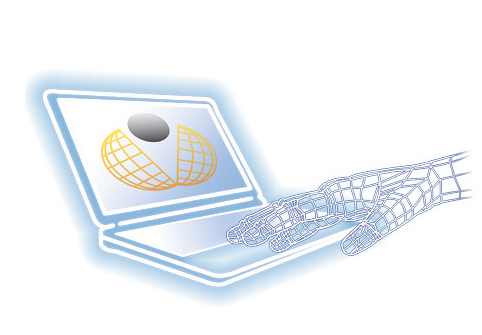
\includegraphics[width=\linewidth]{isima_main.png}
    \vfill \null
  \end{minipage}
  \begin{minipage}[b]{0.89\textwidth}
    \textbf{Institut Supérieur d'Informatique, de Modélisation et de leurs Applications}
    \vskip1mm
    {\color{NavyBlue}\hrule}
    \vskip3mm
    \begin{minipage}{0.78\textwidth}
      \textcolor{NavyBlue}{\large\textbf{www.isima.fr}}\\
      Campus universitaire des Cézeaux -- 1 rue de la Chebarde\\
      TSA 60125 -- CS 60026 -- 63178 Aubière CEDEX\\
      Tel (+33/0) 473 405 000 -- Fax (+33/0) 473 405 001
    \end{minipage}
    \hfill
    \begin{minipage}{0.20\textwidth}
      \raggedleft
      
\includegraphics[height=1.6cm]{UCA_logo.png}
    \end{minipage}
  \end{minipage} 

\end{titlepage}
\makeatother
  \blankpage

  \pagenumbering{roman}       % numérotation en chiffres romains
  
  % Remerciements
  \cleardoublepage
  \null
\vspace{4cm}
\begin{flushright}
	{\Large \bfseries Remerciements}
	\addcontentsline{toc}{chapter}{Remerciements}

	\vspace{1cm}

	\begin{minipage}{0.62\textwidth}
		Nous remercions Christophe Duhamel, responsable de notre projet, pour sa disponibilité tout au long du développement ainsi que pour ses nombreuses explications qui furent d'une aide constante et sans lequelles nous n'aurions pas pu mener ce projet à son terme.
	\end{minipage}

	\vspace{1cm}

	\begin{minipage}{0.62\textwidth}
		Remerciement 2
	\end{minipage}

\end{flushright}


  % Résumé + Abstract sur 1 page
  \cleardoublepage
  \section*{Résumé}
\addcontentsline{toc}{chapter}{Résumé}

L'identification d'objets mobiles est un problème d'optimisation courant pour les tournées de véhicules, doté de nombreuses applications. Par exemple, on peut l'utiliser pour modéliser et organiser des interventions de sécurité ou des opérations humanitaires. Dans les deux cas, le temps est une donnée critique et les solutions doivent maximiser le nombre de mobiles interceptés et minimiser le temps requis total. Ce problème nécessite donc une optimisation bi-critères et est appelé problème sélectif de tournées de véhicules avec dépendance de temps. Pour résoudre ce problème, nous avons implémenté deux heuristiques de construction pour générer des solutions réalisables, mais non optimales. Une politique de cache de données a été réalisée pour accélérer les heuristiques. Ensuite, des procédures de recherche locale ont été ajoutées pour déterminer les améliorations possibles d'une solution et une Vertical Neighbouhood Descent (VND) a été construite pour combiner ces méthodes. Puis deux métaheuristiques fondées sur un algorithme génétique à clés aléatoires et à multiples démarrages ont été utilisées pour générer de meilleures solutions sur les critères de temps et de quantité. Les algorithmes développés doivent être capables de fournir des solutions rapidement, ils ont donc été écrits dans le langage C++ et ont été calibrés avec des problèmes de taille réelle. Nous présentons les résultats de jeux de données connus et générés automatiquement. Les résultats montrent que la politique de cache de données a divisé le temps de calcul des heuristiques par dix. Plusieurs graphiques représentant les données dans l'espace et le temps sont fournis ainsi que le calibrage et la représentation des fronts de Pareto pour la comparaison et le classement des solutions générées. L'efficacité et la convergence des graphiques justifie les décisions stratégiques prises dans le processus de construction de la VND. Les résultats obtenus à la fin du projet confirment que les problèmes de tournées peuvent être résolus en utilisant des méthodes itératives de construction là où une résolution exacte échouerait ou mettrait énormément de temps à cause du très grand nombre de possibilités existantes. Ces résultats nous ont permis de valider une preuve de concept pour la prédiction du temps requis pour arrêter des trafiquants de drogues à bord de véhicules à grande vitesse.

\emph{Mots-clés: Aide à la décision, problème de tournées de véhicules, métaheuristique, Vertical Neighbourhood Descent, optimisation bi-critère.}

\section*{Abstract}
\addcontentsline{toc}{chapter}{Abstract}

Mobile objects identification is a common vehicle routing optimisation problem with several applications. For instance, it can be used to model and organise safety or humanitarian operations. In both cases, time may be critical and solutions must maximise the amount of visited mobiles and minimise the total needed time. This problem needs bi-criteria optimisation and is called an open vehicle routing problem with time dependency. To solve this problem, we implemented two route-building heuristics to generate feasible but not optimal solutions and a memory cache strategy was designed to speed-up the heuristics. Then, local search procedures were coded to look for improvements on the solutions and a Vertical Neighbourhood Descent was built to combine these procedures. After that, two metaheuristics based on a genetic algorithm with random keys and multi-start were used to generate better solutions on both time and amount criteria. The developed algorithms must be able to provide solutions quickly, so they were written using the C++ language and benchmarked with real-size problems. We present results of experiments on self-generated and well-known datasets. Results showed that the memory cache strategy divided the heuristic computation by ten. Several graphical representations for temporal and spatial dimensions were also provided along with a benchmark and Pareto frontiers charts to compare and rank the generated solutions. Efficiency and convergence charts justified the strategic decisions taken in the Vertical Neighbourhood Descent building process. The results obtained at the end of this project confirm that routing problems can be solved using constructive and iterative methods because of the large amount of possibilities on which an exact solver would fail or need an extremely long time to end. These results made it possible for us to validate a proof of concept in predicting how much time is needed to arrest drug smugglers on "go-fast" races.

\emph{Keywords: Decision support, Vehicle Routing Problem, Metaheuristic, Vertical Neighbourhood Descent, Bi-criteria optimisation.}


  % Table des matières, illustrations, tableaux, listings
  \cleardoublepage
  \pagestyle{IHA-fancy-style}
  \newlength{\currentparskip}
\setlength{\currentparskip}{\parskip}
\setlength{\parskip}{0pt}
\tableofcontents

\bigskip\null\bigskip

\noindent\textbf{Nota:} Les termes présents dans le glossaire voient leur première occurrence dans le texte succédée par un double obèle (symbole $\ddagger$).

\newpage
\begingroup
  \addcontentsline{toc}{chapter}{Table des figures}
  \listoffigures
  \addcontentsline{toc}{chapter}{Liste des tableaux}
  \listoftables
  \addcontentsline{toc}{chapter}{Liste des extraits de code}
  \listoflistings
\endgroup
\setlength{\parskip}{\currentparskip}
  \cleardoublepage
  % Mémorisation du dernier numéro de page en chiffres romains
  \newcounter{oldRomanNum}
  \setcounter{oldRomanNum}{\value{page}}
  \pagenumbering{arabic}      % Chiffres arabes

  % Introduction
  \chapter*{Introduction}
\addcontentsline{toc}{chapter}{Introduction}

Ce projet nous a été proposé par Christophe Duhamel, enseignant à l’ISIMA et chercheur au LIMOS.

Il s'inscrit dans la continuité d'un projet réalisé en première année, consistant en une introduction aux problèmes de tournées de véhicules.
Il s'agit d'un problème où les clients sont mobiles et se déplacent selon une trajectoire définie à une vitesse fixe. Au terme de ce premier projet, le calcul d'une seule et unique tournée était réalisable.

Les objectifs liés à ce projet sont multiples. Dans un premier temps, nous avons souhaité adapter les calculs pour permettre la construction de plusieurs tournées. Par la suite nous avons amélioré les résultats fournis par ces calculs de manière à optimiser les tournées selon deux critères: le temps nécessaire pour terminer la tournée la plus longue (en termes de durée), et le nombre total de clients livrés.

La prise en compte de ces deux critères permet d'inscrire le projet dans les conditions qualifiant des problèmes de secours (actions humanitaires) ou de protection des civils (actions militaires). En effet, dans ces deux types de problèmes, le temps est un critère déterminant dans la réactivité et le succès des interventions, et le nombre d'objectifs atteints vise à généraliser ce succès. On peut donc voir à ce projet des utilisations multiples comme l'inspection de sites sensibles, le suivi de déplacements de troupes, l'arrestation de convois de type "go-fast" ou la livraison de matériel de secours, vivres, équipements de première nécessité à des équipes ou des groupes mobiles ou immobiles.

Pour répondre à ces problématiques, nous avons mis en \oe uvre différentes solutions et méthodes de résolution que nous décrirons dans les chapitres suivants. Nous avons attaché une attention particulière à la qualité des résultats, l'optimisation des calculs et la réutilisabilité de notre travail.

Pour des raisons de performances, nos développements ont été réalisés en langage C++, mais les principes que nous évoquerons sont applicables à d'autres langages et paradigmes.

  % Parties
  \chapter{Présentation du sujet}
	\section{Problème}
		Ce problème de tournées de véhicules correspond plus précisément à un STDVRP (\emph{Selective Time-Dependent Vehicle Routing Problem}), c'est-à-dire un problème où tous les clients ne sont pas nécessairement livrés (\emph{Selective}) et où les tournées ne peuvent excéder une certaine durée (Time-Dependent). Cette durée permet par ailleurs de modéliser une autonomie sur ces véhicules. Cela prend d'autant plus de sens si l'on souhaite appliquer ce problème sur une flotte de véhicules autonomes comme des drônes par exemple.

		Afin de fixer certains paramètres nous avons déterminé la nécessité d'utiliser les unités suivantes:
		\begin{itemize}
			\item Unité de temps (u.t.), pour modéliser l'autonomie des véhicules et le temps des tournées,
			\item Unité de distance (u.d.), pour placer les véhicules et les clients,
			\item Unité de vitesse (u.v.), correspondant à une unité de distance par unité de temps, pour calculer les déplacements.
		\end{itemize}

		Nous avons également choisi d'employer certains termes plus en lien avec le sujet. Ainsi les véhicules sont nommés \emph{intercepteurs}, les clients sont nommés \emph{mobiles} et une livraison correspond à une \emph{interception}. Nous avons préféré choisir ces termes car les mobiles sont en mouvement et les intercepteurs doivent changer de direction pour les rejoindre en un même endroit à un même instant, aussi le terme d'interception fait plus de sens.

		Les calculs sont effectués dans le plan (et non dans l'espace). Les coordonnées de différentes entités sont à noter:
		\begin{itemize}
			\item \emph{mobiles}: position initiale (à l'instant $t=0$),
			\item \emph{dépôts}: position fixe
			\item \emph{intercepteurs}: à $t=0$, la position d'un intercepteur est celle du dépôt auquel il est rattaché.
		\end{itemize}

		Chaque mobile et chaque intercepteur avance à une vitesse qui lui est propre. Le mobile doit suivre une direction donnée, et l'intercepteur peut changer de direction après chaque interception.

		L'intercepteur doit rentrer à son dépôt dès la fin de sa tournée, et son autonomie doit lui permettre ce retour. Enfin, la date de fin d'une tournée correspond à la date d'interception du dernier mobile de cette tournée.

		Dans les schémas que nous utiliserons pour décrire nos approches, nous emploierons les symboles suivants:
		\begin{itemize}
			\item Pour un mobile: le symbole (\tikz[baseline=-0.65ex]{\node[mobile,inner sep=0,outer sep=0]{\mobile};}) lorsqu'il est intercepté, ou (\tikz[baseline=-0.65ex]{\node[mobile,uncaught,inner sep=0,outer sep=0]{\mobile};}) lorsqu'il ne l'est pas dans un schéma spatial, et le symbole (\tikz[baseline=-0.65ex]{\node[mobile,draw]{};}) dans un schéma de tournée. Un vecteur vitesse (\tikz[baseline=-0.65ex]{\draw[speed] (0,0) -- (1,0);}) indique sa direction ainsi que sa vitesse. Sa trajectoire est tracée par une ligne pointillée (\tikz[baseline=-0.65ex]{\draw[direction] (0,0) -- (1,0);}).

			\item Pour un dépôt, un symbole (\tikz[baseline=-0.65ex]{\node[interceptor,inner sep=0,outer sep=0]{\interceptor};}) indique sa position.

			\item Pour un intercepteur: son tracé est réalisé en traits pleins, et part d'un dépôt. Afin d'en faciliter la lecture, le retour au dépôt n'est pas représenté. Le tracé est ponctué de symboles (\tikz[baseline=-0.65ex]{\node[route,inner sep=0,outer sep=0]{\mobile};}) aux emplacements où l'interception d'un mobile a eu lieu. La date de fin d'une tournée est indiquée à proximité du dernier mobile intercepté.
		\end{itemize}

		La figure \ref{fig:example} présente un schéma spatial et un schéma de tournée.

		\begin{figure}
			\begin{subfigure}[b]{.45\linewidth}
				\centering
				\begin{tikzpicture}[scale=.5]
					\draw[grided,step=1.0,thin] (0,0) grid (12,12);
\draw[color=Gray] (0,0) -- coordinate (x axis mid) (12,0);
\draw[color=Gray] (0,0) -- coordinate (x axis mid) (0,12);
\foreach \x in {0,...,12}
\draw[color=Gray] (\x,1pt) -- (\x,-3pt) node[anchor=north] {\x};
\foreach \y in {0,...,12}
\draw[color=Gray] (1pt,\y) -- (-3pt,\y) node[anchor=east] {\y};
\node[interceptor] (D0) at (12,12) {\interceptor};
\node (I0) at (D0) {};
\node[interceptor] at ($ (I0) + (315:0.4) $) {$I_0$};
\node[mobile,anchor=center] (M0) at (2,5) {\mobile};
\node[mobile] at (M0.south east) {$M_{0}$};
\draw[speed] (M0.center) -- ($ (M0.center) + (1,0.3) $);
\node[mobile,anchor=center] (M1) at (4,1) {\mobile};
\node[mobile] at (M1.south east) {$M_{1}$};
\draw[speed] (M1.center) -- ($ (M1.center) + (0.5,0.5) $);
\node[mobile,uncaught,anchor=center] (M2) at (6,10) {\mobile};
\node[mobile] at (M2.south east) {$M_{2}$};
\draw[speed,uncaught] (M2.center) -- ($ (M2.center) + (-4,0) $);
\draw[direction] (M0.center) -- (6.11793,6.23538);
\draw[route] (12,12) -- (6.11793,6.23538);
\node[route] at (6.11793,6.23538) {\mobile};
\draw[direction] (M1.center) -- (6.70783,3.70783);
\draw[route] (6.11793,6.23538) -- (6.70783,3.70783);
\node[route] at (6.70783,3.70783) {\mobile};
\draw[route](6.70783,3.70783) node[anchor=north east] {$t_{0}=5.41567$};
				\end{tikzpicture}
				\subcaption{Représentation spatiale}
				\label{subfig:spatial}
			\end{subfigure}
			\hfill
			\begin{subfigure}[b]{.45\linewidth}
				\centering
				\vfill
				\begin{tikzpicture}[schema]
					\begin{scope}[start chain=trunk]
	\node[interceptor, on chain, label=left:$I_0$] {};
	\node[mobile, on chain, join, label=above:$M_0$] {};
	\node[mobile, on chain, join, label=above:$M_1$] {};
	\node[interceptor, on chain, join] {};
\end{scope}
				\end{tikzpicture}
				\vfill
				\null
				\subcaption{Représentation schématique d'une tournée}
			\end{subfigure}
			\caption{Exemples de schémas}
			\label{fig:example}
		\end{figure}

	\section{Etat de l'art}
		\TODO{Demander à C. Duhamel l'avancée de la recherche dans ce domaine.}

		Le projet réalisé en première année permettait de travailler avec un seul intercepteur pour obtenir des résultats comme celui que l'on peut voir sur la figure \ref{subfig:spatial}. Le programme était écrit en langage C et prenait en entrée un fichier décrivant les données du problème. Le listing \ref{lst:old_input_file} correspond au fichier d'entrée menant au résultat de la figure \ref{subfig:spatial}.

		Ce fichier avait été conçu pour en faciliter l'évolution. Bien que le programme ne puisse travailler qu'avec un seul intercepteur, il était possible d'en renseigner plusieurs, ainsi que plusieurs dépôts. Nous avons donc conservé un format de fichier similaire pour notre projet, il sera présenté plus tard.

		\begin{code}
			\textfile{files/old_input_file.txt}
			\captionof{listing}{Fichier d'entrée original}
			\label{lst:old_input_file}
		\end{code}

	\section{Travail à réaliser}
		Notre projet avait pour objectif de réutiliser le travail initial en généralisant les heuristiques de construction pour qu'elles puissent fonctionner avec de multiples intercepteurs, ainsi que d'optimiser les résultats selon deux critères : le nombre de mobiles visités et le temps requis pour l'interception.
Plusieurs étapes étaient nécessaires pour réaliser ce projet.

Tout d'abord, un travail de révision et d'optimisation était requis avant de pouvoir poursuivre ce qui avait été fait. Le code initial ayant été réalisé en langage C, il a été traduit en C++ dans une architecture adaptée et orientée objet. Puis le code obtenu a été adapté pour généraliser le problème à non plus un seul, mais plusieurs intercepteurs pouvant provenir de différents dépôts.

		\begin{figure}[h!]
			\centering
			\begin{tikzpicture}
				\umlclass[anchor=center]{Problem}{
}{
	+ Problem(string)\\
	+ Problem(Problem)\\
	+ nbMobiles() : int\\
	+ nbInterceptors() : int\\
	+ nbDepots() : int\\
	+ mobiles() : vector<Mobile>\\
	+ interceptors() : vector<Interceptor>\\
	+ depots() : vector<Depot>\\
	+ write(string) : void\\
}

\umlclass[x=8.5,y=-4.5,anchor=north]{Interceptor}{
	-- id : int\\
	-- position : Location\\
	-- speed : Speed\\
	-- range : Time\\
	\umlstatic{+ INTERCEPTION\_TIME\_NO\_FUEL : Time}
}{
	+ Interceptor(Location, Speed, int, Time)\\
	+ id() : int\\
	+ position() : Location\\
	+ speed() : Speed\\
	+ range() : Time\\
	+ depot() : Depot\\
	+ position(Location) : void\\
	+ speed(Speed) : void\\
	+ range(Time) : void\\
	+ computeInterception(Location, Mobile, Time) : Time\\
	+ timeFromTo(Location, Location) : Time
}

\umlclass[y=-4.5,anchor=north]{Mobile}{
	-- id : int\\
	-- position : Location\\
	-- direction : Direction\\
}{
	+ Mobile(Location, Direction, int)\\
	+ id() : int\\
	+ position() : Location\\
	+ position(Time) : Location\\
	+ direction() : Direction\\
	+ speed() : Speed\\
	+ position(Location) : void\\
	+ direction(Direction) : void
}

\umlclass[x=8.5,anchor=center]{Depot}{
	-- id : int\\
	-- position : Location\\
}{
	+ Depot(Location, Direction, int)\\
	+ id() : int\\
	+ position() : Location\\
	+ interceptors() : vector<Interceptor>\\
	+ position(Location) : void\\
	+ addInterceptor(Interceptor) : void
}

\umlunicompo[geometry=--,arg=depots, mult1=1, mult2=*]{Problem}{Depot}
\umlunicompo[geometry=--,arg=mobiles, mult1=1, mult2=*]{Problem}{Mobile}
\umlunicompo[geometry=--,arg=interceptors, mult1=1, mult2=*]{Problem}{Interceptor}
\umluniaggreg[geometry=--,arg=interceptors, mult1=1, mult2=*,anchor1=-70, anchor2=70]{Depot}{Interceptor}
\umluniaggreg[geometry=--,arg=depot, mult1=1, mult2=1,anchor1=110, anchor2=-110]{Interceptor}{Depot}
			\end{tikzpicture}
			\caption{Classes définissant un problème}
			\label{fig:problem-uml}
		\end{figure}
\TODO{en cours de rédaction}

		\begin{enumerate}
			\item Porter le code existant (langage C) en C++ dans une architecture adaptée et orientée objet.
			\item Adapter le code pour travailler dans un contexte multi-intercepteurs.
			\item Optimiser ce code.
			\item Revoir les représentations graphiques.
			\item Définir les objectifs d'amélioration des solutions.
			\item Définir des opérations d'amélioration des résultats obtenus (Recherche Locale).
			\item Définir des combinaisons de mouvements améliorants intéressantes.
			\item Appliquer ces mouvements dans le cadre d'une métaheuristique.
			\item Tenir compte de paramètres supplémentaires pour plus de réalisme.
		\end{enumerate}

		Notons que plusieurs mesures sont fixées pour faciliter les calculs:
		\begin{itemize}
			\item Les déplacements se font dans le plan (l'altitude n'a donc pas d'influence).
			\item Les trajectoires des mobiles sont rectilignes, et ils évoluent à vitesse constante.
			\item Les trajectoires des intercepteurs sont suivies à vitesse constante et rectilignes entre deux interceptions consécutives.
		\end{itemize}

		Pour assurer un suivi régulier du projet, nous avons planifié des réunions avec M. Duhamel chaque semaine dans la mesure du possible ou toutes les deux semaines.

		Ainsi nous avons construit le diagramme de Gantt prévisionnel présenté sur la figure \TODO{FIGURE}.

  \chapter{Méthodes}
	\section{Heuristiques constructives}
		Nous proposons deux heuristiques d'insertion. La première est pilotable par l'utilisateur et la seconde est autonome.

		Ces deux heuristiques servent à construire des solutions réalisables. L'optimalité de ces solutions n'est pas garantie et n'est pas un objectif. En effet, une heuristique est une étape de résolution qui vise seulement à produire une solution viable sur laquelle on pourra appliquer des modifications de manière itérative jusqu'à l'obtention d'un résultat répondant aux critères de qualité que l'on aura fixés.

		Il est très souvent plus facile d'améliorer un système dont on sait qu'il fonctionne que de chercher à rendre efficace un système défectueux.
		\subsection{Interception selon une séquence}
		\label{sub:heuristic_sequence}
			Dans cette heuristique, l'utilisateur fournit une séquence de mobiles à intercepter dans l'ordre de la lecture de cette séquence. L'heuristique est alors chargée pour chaque mobile de cette séquence de déterminer l'intercepteur capable de l'atteindre dans les meilleurs délais. On garantit alors la propriété suivante pour chaque tournée $r$:
			\[
				\forall i, j \qtext{t.q.}  i<j, \qtext{on a} \text{pos}(r_i) < \text{pos}(r_j)
			\]
			avec $r_k$ le mobile intercepté en $k$\ieme{} position dans la tournée $r$, et pos($r_k$) la fonction permettant d'obtenir la position du mobile $r_k$ dans la séquence imposée par l'utilisateur.

			La figure~\ref{fig:heuristic_sequence_demo} présente un exemple de solution réalisable.

			\begin{figure}[h!]
			\centering
			Séquence donnée: $\{4, 2, 3, 0, 1\}$

			\begin{tikzpicture}[schema]
				\begin{scope}[start chain=trunk]
	\node[interceptor, on chain, label=left:$I_0$] {};
	\node[mobile, on chain, join, label=above:$M_4$] {};
	\node[mobile, on chain, join, label=above:$M_0$] {};
	\node[interceptor, on chain, join] {};
\end{scope}
\begin{scope}[start chain=trunk,yshift=-1.25cm]
	\node[interceptor, on chain, label=left:$I_1$] {};
	\node[mobile, on chain, join, label=above:$M_2$] {};
	\node[mobile, on chain, join, label=above:$M_3$] {};
	\node[mobile, on chain, join, label=above:$M_1$] {};
	\node[interceptor, on chain, join] {};
\end{scope}

			\end{tikzpicture}
			\caption{Exemple de solution réalisable pour l'heuristique ``Séquence''}
			\label{fig:heuristic_sequence_demo}
			\end{figure}

		\subsection{Interception au plus tôt}
		\label{sub:heuristic_fastest}
			Dans cette heuristique, le calcul de chaque interception est piloté par le temps. L'heuristique calcule pour chaque insertion les meilleurs candidats (mobile et tournée). Il s'agit donc de déterminer quel est le mobile qui pourra être inseré dans la tournée réalisée par l'intercepteur capable de le rejoindre au plus tôt. Il s'agit d'une méthode plus gourmande en ressources, mais qui permet d'obtenir des résultats généralement de meilleure qualité que l'insertion par séquence.

			Afin d'optimiser les performances, nous avons développé une politique de \gls{cache} permettant de conserver une matrice des durées nécessaires pour atteindre chaque mobile à partir de chaque intercepteur. Ainsi, lorsqu'un mobile est intercepté, seules les durées relatives à l'intercepteur candidat sont faussées et doivent être recalculées, les durées nécessaires aux autres intercepteurs pour atteindre les autres mobiles restent identiques. Nous décrivons plus en détail ce mécanisme dans l'annexe~\ref{app:cache}.

			Toutefois, cette heuristique doit être utilisée avec parcimonie en raison de son coût de calcul, mais aussi car elle n'est pas paramétrable et n'offre donc pas de capacité d'extension de ses possibilités, notamment le fait d'ignorer des mobiles ou de prioriser l'interception d'un mobile par rapport à un autre sur une décision arbitraire.

			\begin{figure}[h!]
				\begin{subfigure}[t]{.5\linewidth}
					\centering
					\caption{Au plus tôt}
					\label{subfig:fastest_demo}
					\begin{tikzpicture}[scale=.5,baseline,transform shape]
						\draw[grided,step=1.0,thin] (-3,-2) grid (12,12);
\draw[color=Gray] (-3,0) -- coordinate (x axis mid) (12,0);
\draw[color=Gray] (0,-2) -- coordinate (x axis mid) (0,12);
\foreach \x in {-3,...,12}
\draw[color=Gray] (\x,1pt) -- (\x,-3pt) node[anchor=north] {\x};
\foreach \y in {-2,...,12}
\draw[color=Gray] (1pt,\y) -- (-3pt,\y) node[anchor=east] {\y};
\node[interceptor] (D0) at (0,0) {\interceptor};
\node (I0) at (D0) {};
\node[interceptor] at ($ (I0) + (315:0.4) $) {$I_0$};
\node[interceptor] (D1) at (12,12) {\interceptor};
\node (I1) at (D1) {};
\node[interceptor] at ($ (I1) + (315:0.4) $) {$I_1$};
\node[mobile,anchor=center] (M0) at (1,2) {\mobile};
\node[mobile] at (M0.south east) {$M_{0}$};
\draw[speed] (M0.center) -- ($ (M0.center) + (-1,0) $);
\node[mobile,anchor=center] (M1) at (4,1) {\mobile};
\node[mobile] at (M1.south east) {$M_{1}$};
\draw[speed] (M1.center) -- ($ (M1.center) + (0.5,0.5) $);
\node[mobile,anchor=center] (M2) at (0,3) {\mobile};
\node[mobile] at (M2.south east) {$M_{2}$};
\draw[speed] (M2.center) -- ($ (M2.center) + (0,-1) $);
\node[mobile,anchor=center] (M3) at (2,5) {\mobile};
\node[mobile] at (M3.south east) {$M_{3}$};
\draw[speed] (M3.center) -- ($ (M3.center) + (1,0.3) $);
\node[mobile,anchor=center] (M4) at (-1,-2) {\mobile};
\node[mobile] at (M4.south east) {$M_{4}$};
\draw[speed] (M4.center) -- ($ (M4.center) + (-0.5,0.5) $);
\draw[direction] (M0.center) -- (2.22045e-16,2);
\draw[interceptor] (0,0) -- (2.22045e-16,2);
\node[interceptor] at (2.22045e-16,2) {\mobile};
\draw[direction] (M2.center) -- (0,2);
\draw[interceptor] (2.22045e-16,2) -- (0,2);
\node[interceptor] at (0,2) {\mobile};
\draw[direction] (M4.center) -- (-2.38482,-0.615179);
\draw[interceptor] (0,2) -- (-2.38482,-0.615179);
\node[interceptor] at (-2.38482,-0.615179) {\mobile};
\draw[interceptor](-2.38482,-0.615179) node[anchor=north west] {$t_{0}=2.76964$};
\draw[direction] (M3.center) -- (6.11793,6.23538);
\draw[interceptor] (12,12) -- (6.11793,6.23538);
\node[interceptor] at (6.11793,6.23538) {\mobile};
\draw[direction] (M1.center) -- (6.70783,3.70783);
\draw[interceptor] (6.11793,6.23538) -- (6.70783,3.70783);
\node[interceptor] at (6.70783,3.70783) {\mobile};
\draw[interceptor](6.70783,3.70783) node[anchor=north east] {$t_{1}=5.41567$};

					\end{tikzpicture}
				\end{subfigure}
				\hfill
				\begin{subfigure}[t]{.5\linewidth}
					\centering
					\caption{Par séquence}
					\label{subfig:_sequence_demo}
					\begin{tikzpicture}[scale=.5,baseline,transform shape]
						\tikzset{interceptor/.style = {thick, color=OrangeRed}}
						\draw[grided,step=1.0,thin] (-7,-7) grid (12,12);
\draw[color=Gray] (-7,0) -- coordinate (x axis mid) (12,0);
\draw[color=Gray] (0,-7) -- coordinate (x axis mid) (0,12);
\foreach \x in {-7,...,12}
\draw[color=Gray] (\x,1pt) -- (\x,-3pt) node[anchor=north] {\x};
\foreach \y in {-7,...,12}
\draw[color=Gray] (1pt,\y) -- (-3pt,\y) node[anchor=east] {\y};
\node[interceptor] (D0) at (0,0) {\interceptor};
\node (I0) at (D0) {};
\node[interceptor] at ($ (I0) + (315:0.4) $) {$I_0$};
\node[interceptor] (D1) at (12,12) {\interceptor};
\node (I1) at (D1) {};
\node[interceptor] at ($ (I1) + (315:0.4) $) {$I_1$};
\node[mobile,anchor=center] (M0) at (1,2) {\mobile};
\node[mobile] at (M0.south east) {$M_{0}$};
\draw[speed] (M0.center) -- ($ (M0.center) + (-1,0) $);
\node[mobile,anchor=center] (M1) at (4,1) {\mobile};
\node[mobile] at (M1.south east) {$M_{1}$};
\draw[speed] (M1.center) -- ($ (M1.center) + (0.5,0.5) $);
\node[mobile,anchor=center] (M2) at (0,3) {\mobile};
\node[mobile] at (M2.south east) {$M_{2}$};
\draw[speed] (M2.center) -- ($ (M2.center) + (0,-1) $);
\node[mobile,anchor=center] (M3) at (2,5) {\mobile};
\node[mobile] at (M3.south east) {$M_{3}$};
\draw[speed] (M3.center) -- ($ (M3.center) + (1,0.3) $);
\node[mobile,anchor=center] (M4) at (-1,-2) {\mobile};
\node[mobile] at (M4.south east) {$M_{4}$};
\draw[speed] (M4.center) -- ($ (M4.center) + (-0.5,0.5) $);
\draw[direction] (M0.center) -- (2.22045e-16,2);
\draw[interceptor] (0,0) -- (2.22045e-16,2);
\node[interceptor] at (2.22045e-16,2) {\mobile};
\draw[direction] (M1.center) -- (6.02906,3.02906);
\draw[interceptor] (2.22045e-16,2) -- (6.02906,3.02906);
\node[interceptor] at (6.02906,3.02906) {\mobile};
\draw[direction] (M2.center) -- (0,-6.84105);
\draw[interceptor] (6.02906,3.02906) -- (0,-6.84105);
\node[interceptor] at (0,-6.84105) {\mobile};
\draw[interceptor](0,-6.84105) node[anchor=south east] {$t_{0}=9.84105$};
\draw[direction] (M3.center) -- (6.11793,6.23538);
\draw[interceptor] (12,12) -- (6.11793,6.23538);
\node[interceptor] at (6.11793,6.23538) {\mobile};
\draw[direction] (M4.center) -- (-6.23744,3.23744);
\draw[interceptor] (6.11793,6.23538) -- (-6.23744,3.23744);
\node[interceptor] at (-6.23744,3.23744) {\mobile};
\draw[interceptor](-6.23744,3.23744) node[anchor=north west] {$t_{1}=10.4749$};

					\end{tikzpicture}
				\end{subfigure}
				\caption{Application des heuristiques d'insertion}
				\label{fig:heuristics_demo}
			\end{figure}


	\section{Recherche Locale et optimisation bi-critères}
		La recherche locale vise à améliorer une solution en réalisant une succession de mutations simples. En effet, lorsque l'heuristique d'insertion se termine, deux cas se présentent:
		\begin{itemize}
			\item Tous les mobiles ont été interceptés,
			\item Il reste un ou plusieurs mobiles non-interceptés.
		\end{itemize}

		Dans le premier cas, le moyen le plus simple pour gagner du temps consiste à retirer un mobile, ce mouvement est présenté plus bas. Dans le second cas, on peut essayer d'insérer les mobiles restants dans une tournée (page~\pageref{subs:move_insert}).

		Il est également possible de combiner ces deux mouvements élémentaires pour former quel\-ques mouvements plus complexes, par exemple enlever un mobile pour le déplacer dans une autre tournée, ou ailleurs dans la même tournée. Nous présentons donc plusieurs mouvements que nous jugeons pertinents dans les sections suivantes.

		Il est cependant nécessaire de veiller à ce que les mouvements ainsi décrits soient appliqués stratégiquement, car l'objectif est d'améliorer la solution et non de la détériorer. Il convient donc de fixer les limites d'une détérioration que l'on jugera acceptable. L'intérêt d'autoriser une légère détérioration est que celle-ci ne peut être que temporaire, pour permettre la validation d'un autre mouvement qui laissera ensuite envisager une amélioration plus forte.

		Les objectifs de qualité pour une solution sont le nombre de mobiles interceptés et la date de fin de la tournée la plus longue (en termes de durée). C'est la raison pour laquelle nous avons défini des politiques d'amélioration visant à atteindre ces objectifs qui sont mutuellement contradictoires, tout en garantissant que les limites de détérioration ne soient pas dépassées. Ces politiques définissent quelle est la solution à choisir et valident (ou invalident) des propositions de modification. Elles sont décrites dans la section \ref{subs:first_available_policy}.

		\subsection{Mouvements améliorants}

		Nous présentons ici les mouvements que nous proposons. Ils sont notamment détaillés sur des schémas sur lesquels nous faisons apparaître avec des flèches pleines rouges le mouvement souhaité, et en pointillés les opérations nécessaires (numérotées au besoin).

		\subsubsection{Mouvement d'extraction}
			Le mouvement d'extraction permet de retirer un mobile dans une tournée afin d'améliorer le pire temps d'interception. Pour cela, seule la suppression d'un mobile dans la tournée la plus longue en temps sera validée, car une extraction dans les autres tournées n'apporterait pas d'amélioration globale à la solution. De plus, la pire tournée ne sera pas toujours la même au cours des améliorations successives, donc ce mouvement pourra être appliqué à différentes tournées. 

			Afin que le mouvement ne vide pas successivement les tournées jusqu'à aboutir à une solution où aucun mobile n'est intercepté (solution triviale pour la minimisation du temps), une politique a été ajoutée pour considérer le problème avec le critère de temps, mais aussi celui du nombre de mobiles. Un minimum est donc fixé pour ne pas aller en-dessous d'un certain seuil.
			
			\newpage
			\begin{code}
				\begin{algo}[informal]
					\ALGO{Principe d'extraction d'un mobile dans une tournée}
					\BEGIN
						\STATE{Amélioration ← Faux}
						\STATE{Récupérer la pire tournée t en temps}
						\FORGEN{tous les mobiles m dans la tournée t faire}
							\STATE{Calculer le temps d'interception de la tournée sans le mobile m}
							\IF{le temps d'interception est fini et que la politique est respectée}
								\STATE{Amélioration ← Vrai}
							\ENDIF
						\ENDFORGEN
						\RETURN{Amélioration}
					\END
				\end{algo}
				\captionof{listing}{Algorithme de principe -- Extraction d'un mobile hors d'une tournée}
			\end{code}
			
			\label{subs:move_extract}
			\begin{figure}[h!]
			\centering
			\begin{tikzpicture}[schema]
				\begin{scope}[start chain, x=0,y=0]
	\node[interceptor, on chain] {};
	\node[mobile, on chain, join] {};
	\node[mobile, on chain, join] (B) {};
	\node[mobile, on chain, join,red] (E) {};
	\node[mobile, on chain, join] (A) {};
	\node[interceptor, on chain, join] {};
\end{scope}
\draw[correction,dotted] (B) to[bend right] (A);
\draw[correction] (E) -- ($ (E) + (0,1) $);
\node[right= .5 of B,cross] {$\times$};
\node[right= .5 of E,cross] {$\times$};

			\end{tikzpicture}
			\caption{Schéma d'extraction d'un mobile hors d'une tournée}
			\label{fig:move_extract}
			\end{figure}

		\subsubsection{Mouvement d'insertion}
			Le mouvement d'insertion permet d'ajouter un mobile à une tournée. Il est donc forcément améliorant en termes de mobiles, mais il peut alors impacter le temps maximum d'interception. Ce mouvement sera donc validé uniquement s'il ne l'augmente pas au-delà des limites autorisées.
			
			\begin{code}
				\begin{algo}[informal]
					\ALGO{Principe d'insertion d'un mobile dans une tournée}
					\BEGIN
						\FORGEN{tous les mobiles non interceptés m}
							\FORGEN{toutes les tournées t}
								\FORGEN{toutes les positions p}
									\STATE{Calculer le temps d'interception en insérant m dans t à la position p}
									\IF{l'insertion est possible (le temps est fini)}
										\STATE{Comparer le résultat obtenu avec le temps initial (avec arrêt de la recherche selon les politiques)}
									\ENDIF
								\ENDFORGEN
							\ENDFORGEN
						\ENDFORGEN
						\RETURN{vrai s'il y a eu amélioration, faux sinon}
					\END
				\end{algo}
				\captionof{listing}{Algorithme de principe -- Insertion d'un mobile dans une tournée}
			\end{code}
					
		
			\label{subs:move_insert}
			\begin{figure}[h!]
			\centering
			\begin{tikzpicture}[schema]
				\begin{scope}[start chain,x=0,y=0]
	\node[interceptor, on chain] {};
	\node[mobile, on chain, join] {};
	\node[mobile, on chain, join] (B) {};
	\node[mobile, on chain, join] (A) {};
	\node[mobile, on chain, join] {};
	\node[interceptor, on chain, join] {};
\end{scope}
\node[right= .5 of B,cross] (X) {$\times$};
\node[mobile, below= .5 of X,red] (I) {};
\draw[correction,dotted] (B) -- (I);
\draw[correction,dotted] (I) -- (A);

			\end{tikzpicture}
			\caption{Schéma d'insertion d'un mobile dans une tournée}
			\label{fig:move_insert}
			\end{figure}

		\subsubsection{Mouvement de substitution (ou remplacement)}
				Le mouvement de substitution permet d'insérer un mobile à la place d'un autre mobile dans une tournée. Il s'agit donc d'un mouvement de suppression suivi d'un mouvement d'insertion. Comme le nombre de mobiles ne change pas, seul le gain de temps est considéré pour valider ou non l'opération.
				
				L'algorithme de principe est le suivant :
				\begin{code}
					\begin{algo}[informal]
						\ALGO{Principe du remplacement dans une tournée}
						\BEGIN
							\FORGEN{tous les mobiles non interceptés m}
								\FORGEN{toutes les tournées t}
									\FORGEN{tous les mobiles m' dans t}
										\STATE{Calculer le temps d'interception en remplaçant m' par m dans t}
										\STATE{Comparer le résultat obtenu avec le temps initial (avec arrêt de la recherche selon les politiques)}
									\ENDFORGEN
								\ENDFORGEN
							\ENDFORGEN
							\RETURN{vrai s'il y a eu amélioration, faux sinon}
						\END
					\end{algo}
				\captionof{listing}{Algorithme de principe -- Remplacement d'un mobile dans une tournée}
			\end{code}
			
			\begin{figure}[h!]
			\centering
			\begin{tikzpicture}[schema]
				\begin{scope}[start chain]
	\node[interceptor, on chain] {};
	\node[mobile, on chain, join] {};
	\node[mobile, on chain, join] (B) {};
	\node[mobile, on chain, join,red] (R) {};
	\node[mobile, on chain, join] (A){};
	\node[interceptor, on chain, join] {};
\end{scope}
\node[right= .5 of B,cross] (X) {$\times$};
\node[right= .5 of R,cross] {$\times$};
\node[mobile, below= .5 of R,red] (I) {};
\draw[correction,dotted] (B) -- (I);
\draw[correction,dotted] (I) -- (A);
\draw[correction] (R) -- ($ (R) + (0,1) $);

			\end{tikzpicture}
			\caption{Schéma de substitution d'un mobile dans une tournée}
			\label{fig:move_replace}
			\end{figure}

		\subsubsection{Mouvements de déplacement}
			Le mouvement de déplacement d'un mobile dans une tournée consiste à changer de position l'un des mobiles au sein de la même tournée. L'objectif est de trouver une meilleure organisation de la tournée et donc d'obtenir un gain de temps sur la date d'interception finale.
			Le mouvement de déplacement d'un mobile dans une autre tournée consiste à supprimer un mobile de sa tournée pour l'insérer dans une seconde tournée.

			Les algorithmes de principe sont les suivants:
			\begin{code}
				\begin{algo}[informal]
					\ALGO{Principe du déplacement dans une tournée}
					\BEGIN
						\FORGEN{toutes les tournées t}
							\FORGEN{toutes les positions p possibles dans t}
								\FORGEN{tous les mobiles m}
									\IF{le déplacement existe}
										\STATE{Calculer le nouveau temps d'interception de t avec le déplacement de m dans la tournée.}
										\STATE{Comparer le résultat obtenu avec le temps initial (politiques)}
									\ENDIF
								\ENDFORGEN
							\ENDFORGEN
						\ENDFORGEN
						\RETURN{vrai s'il y a eu amélioration, faux sinon}
					\END
				\end{algo}
				\captionof{listing}{Algorithme de principe -- Déplacement au sein d'une tournée}
			\end{code}

			\begin{code}
				\begin{algo}[informal]
					\ALGO{Principe du déplacement dans deux tournées}
					\BEGIN
						\FORGEN{toutes les tournées t1}
							\FORGEN{tous les mobiles m dans t1}
								\FORGEN{toutes les tournées t2}
									\FORGEN{toutes les positions dans t2}
										\STATE{Calculer le nouveau temps d'interception de t2 avec l'insertion de m à la position p}
										\STATE{Comparer le résultat obtenu avec le temps inital (politiques)}
									\ENDFORGEN
								\ENDFORGEN
							\ENDFORGEN
						\ENDFORGEN
						\RETURN{vrai s'il y a eu amélioration, faux sinon}
					\END
				\end{algo}
				\captionof{listing}{Algorithme de principe -- Déplacement d'un mobile vers une autre tournée}
			\end{code}

			\begin{figure}[h!]
			\begin{subfigure}[b]{.54\linewidth}
				\centering
				\begin{tikzpicture}[schema]
					\begin{scope}[start chain]
	\node[interceptor, on chain] {};
	\node[mobile, on chain, join] (B) {};
	\node[mobile, on chain, join,red] (M) {};
	\node[mobile, on chain, join] (A) {};
	\node[mobile, on chain, join] (I) {};
	\node[mobile, on chain, join] (IA) {};
	\node[interceptor, on chain, join] {};
\end{scope}
\draw[correction,dotted] (B) to[bend right] node[stepnode] {1} (A);
\draw[correction,dotted] (I) to[bend right] node[stepnode] {2} (M);
\draw[correction,dotted] (M) to[bend left, out=60, in=120] node[stepnode] {3} (IA);
\node[right= .5 of M,cross] {$\times$};
\node[right= .5 of B,cross] {$\times$};
\node[right= .5 of I,cross] (X) {$\times$};
\draw[correction] (M) to[bend right] (X);

				\end{tikzpicture}
				\subcaption{Au sein d'une même tournée}
				\label{subfig:move_move1route}
			\end{subfigure}
			\hfill
			\begin{subfigure}[b]{.45\linewidth}
				\centering
				\begin{tikzpicture}[schema]
					\begin{scope}[start chain]
	\node[interceptor, on chain] {};
	\node[mobile, on chain, join] (B) {};
	\node[mobile, on chain, join,red] (M) {};
	\node[mobile, on chain, join] (A) {};
	\node[interceptor, on chain, join] {};
\end{scope}
\begin{scope}[start chain, yshift=-1.25cm]
	\node[interceptor, on chain] {};
	\node[mobile, on chain, join] {};
	\node[mobile, on chain, join] (I) {};
	\node[mobile, on chain, join] (IA) {};
	\node[mobile, on chain, join] {};
	\node[interceptor, on chain, join] {};
\end{scope}
\draw[correction,dotted] (I) -- node[stepnode] {1} (M);
\draw[correction,dotted] (M) -- node[stepnode] {2} (IA);
\draw[correction,dotted] (B) to[bend left] node[stepnode] {3} (A);
\node[right= .5 of M,cross] {$\times$};
\node[right= .5 of B,cross] {$\times$};
\node[right= .5 of I,cross] (X) {$\times$};
\draw[correction] (M) -- (X);


				\end{tikzpicture}
				\subcaption{Entre deux tournées}
				\label{subfig:move_move2routes}
			\end{subfigure}
			\caption{Schémas de déplacement d'un mobile}
			\label{fig:move_move}
			\end{figure}

		\subsubsection{Mouvements d'interversion (ou swap)}
			Le mouvement d'interversion ou \emph{swap} consiste à échanger deux mobiles déjà présents dans une tournée. Il existe deux variantes de ce mouvement : lorsque les deux mobiles appartiennent à la même tournée ou lorsque les tournées sont différentes. Étant donné que ce mouvement ne peut pas diminuer le nombre de mobiles traités, le critère d'amélioration porte uniquement sur la réduction du temps cumulé des tournées considérées, sous réserve de ne pas excéder pour chacune le temps de la pire tournée.

			L'algorithme de principe pour l'interversion dans une même tournée est le suivant:
			\begin{code}
				\begin{algo}[informal]
					\ALGO{Principe de l'interversion dans une tournée}
					\BEGIN
						\FORGEN{toutes les tournées t}
							\FORGEN{tous les mobiles m1 dans t}
								\FORGEN{tous les mobiles m2 après m1 dans t}
									\STATE{Calculer la nouvelle date finale de t avec m2 à la place de m1}
									\STATE{Comparer le résultat obtenu avec le temps initial (avec arrêt de la recherche selon les politiques)}
								\ENDFORGEN
							\ENDFORGEN
						\ENDFORGEN
						\RETURN{vrai s'il y a eu amélioration, faux sinon}
					\END
				\end{algo}
				\captionof{listing}{Algorithme de principe -- Interversion au sein d'une même tournée}
			\end{code}

			\begin{figure}[h!]
			\begin{subfigure}[b]{.54\linewidth}
				\centering
				\begin{tikzpicture}[schema]
					\begin{scope}[start chain]
	\node[interceptor, on chain] (B1) {};
	\node[mobile, on chain, join,red] (S1) {};
	\node[mobile, on chain, join] (A1) {};
	\node[mobile, on chain, join] (B2) {};
	\node[mobile, on chain, join,red] (S2) {};
	\node[mobile, on chain, join] (A2) {};
	\node[interceptor, on chain, join] {};
\end{scope}
\draw[correction,dotted] (B1) to[bend right] node[stepnode] {1} (S2);
\draw[correction,dotted] (S2) to[bend right] node[stepnode] {2} (A1);
\draw[correction,dotted] (B2) to[bend left] node[stepnode] {3} (S1);
\draw[correction,dotted] (S1) to[bend left,out=60, in=120] node[stepnode] {4} (A2);
\node[left= .5 of S1,cross] {$\times$};
\node[right= .5 of S1,cross] {$\times$};
\node[left= .5 of S2,cross] {$\times$};
\node[right= .5 of S2,cross] {$\times$};
\draw[correction,<->] (S1) to[bend left,out=45,in=135] (S2);

				\end{tikzpicture}
				\subcaption{Au sein d'une même tournée}
				\label{subfig:move_swap1route}
			\end{subfigure}
			\hfill
			\begin{subfigure}[b]{.45\linewidth}
				\centering
				\begin{tikzpicture}[schema]
					\begin{scope}[start chain]
	\node[interceptor, on chain] {};
	\node[mobile, on chain, join] (B1) {};
	\node[mobile, on chain, join,red] (S1) {};
	\node[mobile, on chain, join] (A1) {};
	\node[interceptor, on chain, join] {};
\end{scope}
\begin{scope}[start chain,yshift=-1.25cm]
	\node[interceptor, on chain] {};
	\node[mobile, on chain, join] (B2) {};
	\node[mobile, on chain, join,red] (S2) {};
	\node[mobile, on chain, join] (A2) {};
	\node[interceptor, on chain, join] {};
\end{scope}
\draw[correction,dotted] (B1) -- node[stepnode] {1} (S2);
\draw[correction,dotted] (S2) -- node[stepnode] {2} (A1);
\draw[correction,dotted] (B2) to[out=120,in=-120] ($(B1)+(-1,.5)$) to[out=45,in=135]  node[stepnode,near start] {3} (S1);
\draw[correction,dotted] (S1) to[out=45,in=120] node[stepnode,near end] {4} ($(A1)+(1,.5)$) to[out=-60,in=60] (A2);
\node[left= .5 of S1,cross] {$\times$};
\node[right= .5 of S1,cross] {$\times$};
\node[left= .5 of S2,cross] {$\times$};
\node[right= .5 of S2,cross] {$\times$};
\draw[correction,<->] (S1) -- (S2);

				\end{tikzpicture}
				\subcaption{Entre deux tournées}
				\label{subfig:move_swap2routes}
			\end{subfigure}
			\caption{Schémas d'interversion de deux mobiles}
			\label{fig:move_swap}
			\end{figure}

			\newpage
			L'algorithme de principe pour l'interversion avec deux tournées est le suivant :
			\begin{code}
				\begin{algo}[informal]
					\ALGO{Principe de l'interversion entre deux tournées}
					\BEGIN
						\FORGEN{toutes les tournées t1 sauf la dernière}
							\FORGEN{toutes les tournées t2 après t1}
								\FORGEN{tous les mobiles m1 dans t1}
									\FORGEN{tous les mobiles m2 dans t2}
										\STATE{Calculer le nouveau temps d'interception de t1 avec m2 à la place de m1}
										\STATE{Calculer le nouveau temps d'interception de t2 avec m1 à la place de m2}
										\STATE{Comparer les résultats obtenus avec les temps initiaux (avec arrêt de la recherche selon les politiques)}
									\ENDFORGEN
								\ENDFORGEN
							\ENDFORGEN
						\ENDFORGEN
						\RETURN{vrai s'il y a eu amélioration, faux sinon}
					\END
				\end{algo}
				\captionof{listing}{Algorithme de principe -- Interversion entre deux tournées}
			\end{code}

		\subsubsection{Mouvement d'interversion de fins de tournées (ou 2-Opt)}
			Le mouvement d'interversion de fins de tournées ou 2-Opt consiste à échanger deux séquences de mobiles dans deux tournées différentes. Les séquences considérées sont une suite de mobiles tels qu'ils ont été définis au sein d'une tournée, qu'il s'agisse de la tournée entière ou d'un ensemble à partir d'un mobile donné jusqu'à la fin de la tournée. Comme pour le mouvement d'interversion, le nombre de mobiles ne sera jamais réduit, seul le gain en temps est donc considéré. Un cas particulier de ce mouvement consiste à changer les intercepteurs de chaque tournée.

			\begin{figure}[h!]
			\centering
			\begin{tikzpicture}[schema]
				\begin{scope}[start chain]
	\node[interceptor, on chain] {};
	\node[mobile, on chain, join] (B1) {};
	\node[mobile, on chain, join] (S1) {};
	\node[mobile, on chain, join] (A1) {};
	\node[mobile, on chain, join] (L1) {};
	\node[interceptor, on chain, join] (E1) {};
\end{scope}
\begin{scope}[start chain,yshift=-1.25cm]
	\node[interceptor, on chain] {};
	\node[mobile, on chain, join] (B2) {};
	\node[mobile, on chain, join] (S2) {};
	\node[mobile, on chain, join] (A2) {};
	\node[mobile, on chain, join] (L2) {};
	\node[interceptor, on chain, join] (E2) {};
\end{scope}
\draw[correction,rounded corners] ($(A1) + (-.4,.3)$) rectangle ($(L1) + (.3,-.3) $);
\draw[correction,rounded corners] ($(A2) + (-.4,.3)$) rectangle ($(L2) + (.3,-.3) $);
\draw[correction,dotted] (S1) -- node[stepnode,near start] {1} (A2);
\draw[correction,dotted] (S2) -- node[stepnode,near start] {3} (A1);
\draw[correction,dotted] (L1) -- node[stepnode,near start] {4} (E2);
\draw[correction,dotted] (L2) -- node[stepnode,near start] {2} (E1);
\node[right= .5 of S1,cross] {$\times$};
\node[right= .5 of S2,cross] {$\times$};
\node[right= .5 of L1,cross] {$\times$};
\node[right= .5 of L2,cross] {$\times$};

\draw[correction,<->] ($(L1) + (-.75,-.32) $) -- ($(L2) + (-.75,.32) $);

			\end{tikzpicture}
			\caption{Schéma d'interversion de fins de tournées}
			\label{fig:move_2opt}
			\end{figure}

			\newpage
			L'algorithme de principe pour le mouvement 2-Opt est le suivant :
			\begin{code}
				\begin{algo}[informal]
					\ALGO{Principe du 2-Opt}
					\BEGIN
						\FORGEN{toutes les tournées t1 sauf la dernière}
							\FORGEN{toutes les tournées t2 après t1}
								\FORGEN{tous les mobiles m1 dans t1}
									\FORGEN{tous les mobiles m2 dans t2}
										\STATE{Calculer le nouveau temps d'interception de t1 en remplaçant la séquence [m1 à fin de tournée] par [m2 à fin de tournée]}
										\STATE{Calculer le nouveau temps d'interception de t2 en remplaçant la séquence [m2 à fin de tournée] par [m1 à fin de tournée]}
										\STATE{Comparer les résultats obtenus avec les temps initiaux (avec arrêt de la recherche selon les politiques)}
									\ENDFORGEN
								\ENDFORGEN
							\ENDFORGEN
						\ENDFORGEN
						\RETURN{vrai s'il y a eu amélioration, faux sinon}
					\END
				\end{algo}
				\captionof{listing}{Algorithme de principe -- 2-Opt}
			\end{code}


		\subsection{Recherche locale à travers la VND}

			La mise en place d'une \acrlong{vnd} permet d'automatiser l'utilisation de chacun des mouvements qui ont été définis précédemment sur une solution déjà construite (figure~\ref{uml:vnd}). Le principe consiste à tester chaque mouvement sur la solution pour voir si des améliorations sont possibles et les appliquer le cas échéant. Si l'on ne trouve pas d'amélioration pour un mouvement, on passe alors au mouvement suivant, mais si l'on trouve une amélioration, on reprend dans ce cas la liste des mouvements depuis le début, car il est tout à fait possible que certains mouvements qui n'étaient pas réalisables le soient désormais. 
			
			\begin{figure}[h!]
				\centering
				\begin{tikzpicture}
					\umlclass[anchor=center,template={max\_itr}]{VND}{
}{
   + VND()\\
   + VND(list: vector<Move>)\\
   + movements(): vector<Move>\\
   + run(s: Solution): void\\
   + before(s: Solution): void\\
   + after(s: Solution): void
}

\umlemptyclass[type=abstract, x=6]{Move}

\umluniaggreg[geometry=--,arg=list, mult1=1, mult2=*]{VND}{Move}

				\end{tikzpicture}
				\caption[UML -- VND]{Vertical Neighbourhood Descent}
				\label{uml:vnd}
			\end{figure}

			\begin{code}
				\begin{algo}[informal]
					\ALGO{Principe de la VND}
					\VAR
						\DECLVAR{list}{vector<Move *>}
					\ENDVAR
					\BEGIN
						\STATE{unsigned k=0}
						\REPEAT
							\IF{list[k].scan(solution) == true}
								\STATE{list[k].commit(solution)}
								\STATE{k=0}
							\ELSE
								\STATE{++k}
							\ENDIF
						\ENDREPEAT{k < list.size()}
					\END
				\end{algo}
				\captionof{listing}{Algorithme de principe -- VND}
			\end{code}
			
			\subsubsection{Calibrage de la VND}
				Nous nous sommes vite aperçus que la \acrshort{vnd} était sensible à l'ordre d'application des mouvements de la recherche locale. Par conséquent, nous avons jugé utile de réaliser un calibrage (ou \emph{benchmark}) afin de déterminer des combinaisons intéressantes en termes de vitesse de convergence et de qualité des résultats. Pour ce faire, nous avons défini les différentes possibilités: 8~mouvements différents, pilotables indépendamment par deux politiques (voir section suivante), soit 16 variantes. Nous avons décidé d'inclure systématiquement chaque mouvement. Cela donne une combinaison à 8 mouvements, chacun piloté par une politique. Le nombre de combinaisons possibles s'élève à $16 \times 14 \times 12 \times 10 \times 8 \times 6 \times 4 \times 2 = \np{10321920}$. Il est évidemment impossible de tester toutes ces combinaisons dans un temps raisonnable.

				Nous avons donc opté pour une méthode non exhaustive, en générant aléatoirement des combinaisons. Afin de faciliter le codage, nous avons réalisé une structure proche d'une fabrique, sous forme d'un tableau de foncteurs. Ainsi, en associant à chaque mouvement un indice, il suffit de mélanger aléatoirement ces indices pour obtenir un ordre et de choisir aléatoirement une politique pour chaque mouvement.

				A l'exécution, chaque combinaison aléatoirement générée est appliquée successivement sur plusieurs instances du problème, générées aléatoirement. Les résultats obtenus sont stockés et associés à la combinaison dont ils sont issus.

				Finalement, les résultats sont triés et les combinaisons qui ont mené aux meilleurs d'entre-eux sont extraites. On peut alors analyser ces combinaisons et retenir celles qui apparaissent dans les meilleurs résultats d'un maximum d'instances.

				Nous avons remarqué à l'issue de ce calibrage que le nombre d'itérations de la VND n'avait pas toujours besoin d'être important. Généralement, de bonnes solutions sont obtenues en 30 à 50 itérations, c'est la raison pour laquelle nous avons défini la valeur par défaut de ce maximum à 30, mais elle reste personnalisable (template C++).

				Nous présentons quelques résultats dans l'annexe~\ref{ann:benchmark-vnd}.

				Il s'agit d'un calibrage simple, qui n'est sans doute pas exempt de défauts. Par exemple les mouvements qui favorisent l'amélioration du critère \emph{nombre de mobiles} sont peu nombreux. En effet, seul le mouvement d'insertion permet une amélioration sur ce critère. Il pourrait alors être nécessaire de le faire apparaître plusieurs fois dans un autre type de combinaisons afin d'offrir un meilleur équilibre entre les deux critères.

		\subsection{Politiques d'amélioration}
			Afin de rendre les recherches plus pertinentes ou plus rapides, nous avons proposé des politiques permettant de piloter la validation d'une solution comme étant satisfaisante et de commander l'arrêt ou la poursuite des recherches pour trouver un mouvement améliorant. Ces politiques s'appliquent donc à la recherche locale et sont décrites sur le diagramme UML de la figure~\ref{uml:available-policies}.

			Nous tenons compte, pour valider (ou invalider) un mouvement, de bornes entrant dans le cadre de l'optimisation bi-critères. Un mouvement est considéré comme valide s'il n'implique pas de dépassement de ces bornes. 

			Les bornes concernent les deux critères suivants: \emph{nombre de mobiles interceptés} et \emph{date de fin de la pire tournée}. Elles sont gérées par l'utilisateur ou par le programme et peuvent être fixées pour atteindre ou dépasser un objectif non-négociable ou bien pour relaxer l'une ou l'autre, ou bien chacune des deux contraintes, jusqu'à un seuil choisi.

			Le principe de validation d'un mouvement est simple: il suffit de fournir à la politique les nouvelles valeurs de l'évaluation ainsi que les références que l'on refuse de dépasser. Ces références peuvent dans un premier temps être initialisées aux bornes que nous venons d'évoquer. En cas d'amélioration valide, la politique met à jour les références. Toutefois, elle ne modifie pas les bornes.

			\subsubsection{Politique du premier améliorant}
				\label{subs:first_available_policy}
				Cette politique demande l'arrêt des calculs dès lors qu'elle valide la première combinaison qui permet une amélioration au sens de l'optimisation bi-critères. 

				Elle offre des performances intéressantes en termes de vitesse d'exécution, car elle permet de fournir une solution réalisable et améliorante tout en évitant de tester de nombreuses autres combinaisons.

			\subsubsection{Politique du meilleur améliorant}
				\label{subs:best_available_policy}
				Cette politique, contrairement à la précédente, nécessite de tester toutes les combinaisons possibles pour ne garder que la meilleure. 

				Elle ne demande donc jamais l'arrêt des calculs, mais valide chaque amélioration plus intéressante que la meilleure des précédentes. La recherche se termine quand toutes les combinaisons ont été testées. Dès lors, la meilleure combinaison possible est connue, si elle existe, et peut être validée.

				\begin{figure}[h!]
					\centering
					\begin{tikzpicture}
						\umlclass[anchor=center,type=abstract]{AvailablePolicy}{
	\umlstatic{-- max\_acceptable\_time: Time}\\
 	\umlstatic{-- min\_acceptable\_count: int}
}{
	\umlstatic{+ maxAcceptableTime(): Time}\\
   	\umlstatic{+ minAcceptableCount(): int}\\
	\umlvirt{\umlstatic{+ keepOn(): bool}}\\
   	\umlvirt{\umlstatic{+ reset() : void}}\\
   	\umlvirt{\umlstatic{+ update(time, timeRecord) : bool}}\\
   	\umlvirt{\umlstatic{+ update(time, timeRecord, count, countRecord) : bool}}\\
}

\umlclass[anchor=center, x=-4, y=-6]{BestAvailablePolicy}{
	\umlstatic{-- keepOn: const bool = true}
}{
	\umlstatic{+ keepOn(): bool}\\
   	\umlstatic{+ reset() : void}\\
   	\umlstatic{+ update(time, timeRecord) : bool}\\
   	\umlstatic{+ update(...) : bool}\\
}

\umlclass[anchor=center, x=4, y=-6]{FirstAvailablePolicy}{
	\umlstatic{-- keepOn: bool}
}{
	\umlstatic{+ keepOn(): bool}\\
   	\umlstatic{+ reset() : void}\\
   	\umlstatic{+ update(time, timeRecord) : bool}\\
   	\umlstatic{+ update(...) : bool}\\
}

\umlVHVinherit{BestAvailablePolicy}{AvailablePolicy};
\umlVHVinherit{FirstAvailablePolicy}{AvailablePolicy};
					\end{tikzpicture}
					\caption[UML -- Politiques d'amélioration]{Politiques d'amélioration}
					\label{uml:available-policies}
				\end{figure}


	\section{Métaheuristiques}

		La recherche locale permet d'obtenir de bonnes améliorations au sein d'une solution déterminée, mais les \glspl{algorithme genetique} ajoutent la possibilité d'étendre la recherche de la meilleure solution à une multitude de solutions possibles.

		Les \glspl{algorithme genetique} vont provoquer une perturbation (mutation) dans la solution étudiée, perturbation qui va définir une population sur laquelle on va appliquer la recherche locale. Seuls les meilleurs résultats sont conservés et on réitère l'opération autant de fois que désiré.

		\subsection{Multi-Start Evolutionary Local Search}

			L'algorithme \acrlong{msels} (ou MS-ELS) est la première métaheuristique à avoir été implémentée pour notre solution. Le Multi-Start consiste à créer un certain nombre de solutions aléatoires à partir du problème et sur lesquelles on va appliquer une recherche locale de type ELS. La génération des solutions se fait à partir de l'heuristique de construction séquentielle dont la séquence des mobiles donnée va être aléatoire.

			Puis l'Evolutionary Local Search va, pour un nombre d'itérations donné, perturber la solution avant d'y appliquer la recherche locale. On va alors sélectionner le meilleur résultat local trouvé et relancer l'ELS à de multiples reprises pour déterminer un record parmi le meilleur résultat local de chaque ELS.

			À la fin des itérations du Multi-Start et de l'ELS, l'algorithme retourne la meilleure solution trouvée.

			Nous avons implémenté cette métaheuristique de manière générique (figure~\ref{uml:ms-els}) de manière à ce qu'elle soit réutilisable.

			Algorithme de principe:
			\begin{code}
				\begin{algo}[informal]
					\ALGO{Principe du Multi-Start Evolutionary Local Search}
					\BEGIN
						\FOR{i}{1}{nombre max de générations}
							\STATE{Créer une solution aléatoire}
							\STATE{Record ← solution}
							\FOR{j}{1}{nombre max d'itérations de l'ELS}
								\STATE{Meilleur local ← solution}
								\FOR{k}{1}{nombre max de copies}
									\STATE{Créer une copie de solution}
									\STATE{Créer une perturbation dans la copie (shake)}
									\STATE{Lancer la VND pour la copie}
									\IF{la copie donne un meilleur résultat}
										\STATE{Meilleur local ← copie}
									\ENDIF
								\ENDFOR
								\IF{le meilleur local donne un meilleur résultat que le record}
									\STATE{Record ← meilleur local}
								\ENDIF
							\ENDFOR
						\ENDFOR
						\RETURN{record}
					\END
				\end{algo}
				\captionof{listing}{Algorithme de principe -- MS-ELS}
			\end{code}
			\newpage

			\begin{figure}[H]
				\centering
				\begin{tikzpicture}[node distance=1cm]
					\node (start) [startstop] {Début};
\node (dec2) [decision, below of=start, yshift=-1cm] {Fin ELS ?};
\node (pro3) [process, below of=dec2, yshift=-1cm] {Solution courante};
\node[dispatch, below of=pro3] (explode) {};
\node (copy2) [process, below of=explode] {Copie 2};
\node (copy1) [process, left= 1cm of copy2] {Copie 1};
\node (copyn) [process, right= 1cm of copy2] {Copie n};
\node (zombie1) [process, below of=copy1] {Mutant 1};
\node (zombie2) [process, below of=copy2] {Mutant 2};
\node (zombien) [process, below of=copyn] {Mutant n};
\node (ls1) [process, below of=zombie1] {Local Search 1};
\node (ls2) [process, below of=zombie2] {Local Search 2};
\node (lsn) [process, below of=zombien] {Local Search n};
\node (implode) [dispatch, below of=ls2] {};
\node (best) [process, below of=implode, yshift=-.5cm] {Garder le meilleur};
\node (record) [process, below of=best, yshift=-.5cm] {Actualiser le record};
\node (stop) [startstop, left= 1cm of dec2] {Fin};

\draw [arrow] (start) -- (dec2);
\draw [arrow] (dec2) -- node[anchor=east] {non} (pro3);
\draw [arrow] (dec2.west) -- node[anchor=south] {oui} (stop);
\draw [arrow] (pro3) -- (explode);
\draw [arrow] (explode) -- (copy1.north);
\draw [arrow] (explode) -- (copy2.north);
\draw [arrow] (explode) -- (copyn.north);
\draw [arrow] (copy1) -- (zombie1);
\draw [arrow] (copy2) -- (zombie2);
\draw [arrow] (copyn) -- (zombien);
\draw [arrow] (zombie1) -- (ls1);
\draw [arrow] (zombie2) -- (ls2);
\draw [arrow] (zombien) -- (lsn);
\draw [arrow] (ls1.south) -- (implode);
\draw [arrow] (ls2.south) -- (implode);
\draw [arrow] (lsn.south) -- (implode);
\draw [arrow] (implode) -- (best);
\draw [arrow] (best) -- (record);
\draw [arrow] (record.south) |- ++(7,-.5) |- (dec2.east);

				\end{tikzpicture}
				\caption{Logigramme pour le MS-ELS}
				\label{fig:ms-els-logigram}
			\end{figure}

			\begin{figure}[H]			
				\centering
				\begin{tikzpicture}
					\umlclass[anchor=center,template={it\_ms, it\_els, copies, LS, Pb, Sol, Cmp<Sol>},alias=msels,width=7cm]{MS\_ELS}{
}{
   + MS\_ELS()\\
   + run(s: Pb): Sol
}

\umlnote[x=8,y=-2.5,width=6cm]{msels}{
	\begin{description}
		\item[it\_ms]{Nombre d'itérations multi-start}
		\item[it\_els]{Nombre d'itérations ELS}
		\item[copies]{Nombre de copies}
		\item[LS]{Recherche Locale}
		\item[Pb]{Problème}
		\item[Sol]{Solution}
		\item[Cmp<Sol>]{Comparateur de Solution}
	\end{description}}
				\end{tikzpicture}
				\caption[UML -- Métaheuristique MS-ELS]{Classe MS-ELS}
				\label{uml:ms-els}
			\end{figure}

		\subsection{Biased Random-Key Genetic Algorithm}
			\Gls{brkga} est un \gls{algorithme genetique} basé sur un système de vecteurs de clés aléatoires. Un vecteur est un chromosome constitué de $n$ allèles. BRKGA dispose d'une population de $m$ chromosomes. Par l'intermédiaire d'un décodeur, on transforme ces chromosomes en solutions répondant à un problème. Ces solutions sont ensuite évaluées et la valeur obtenue décrit la pertinence du chromosome. Les meilleurs chromosomes sont considérés comme l'élite de la population. BRKGA fait évoluer sa population de chromosomes au cours du temps: plusieurs opérations sont possibles comme la conservation à l'identique, la mutation, ou encore le remplacement par un autre chromosome. A terme, on obtient un ensemble de bons chromosomes qui mènent à des solutions de bonne qualité. On peut également choisir de ne retenir que le meilleur chromosome.

			Dans notre cas, il s'agissait de générer des solutions d'interceptions à un problème donné. Nous avons donc réutilisé l'heuristique d'insertion par séquence, en conservant toutes les étapes de construction, pour générer un ensemble de solutions pour chaque chromosome.
			Le décodage du chromosome en une séquence d'interception se fait de la manière suivante (les clés du chromosome sont des réels entre 0 et 1):
			\begin{itemize}
				\item On trie le chromosome par ordre croissant,
				\item On associe à chaque mobile du problème la valeur située à la même position dans le chromosome trié,
				\item On place chaque mobile dans la séquence selon l'ordre initial du chromosome.
			\end{itemize}
			Cela implique que la taille d'un chromosome doit être identique au nombre de mobiles du problème.

			Pour évaluer la pertinence d'un chromosome, nous observons les solutions qui lui correspondent. Il s'agit donc d'un ensemble de compromis entre nombre de mobiles interceptés et temps nécessaire pour la tournée la plus longue. Nous sommes par conséquent dans un contexte bi-critères, ce qui permet de travailler sur des fronts de Pareto pour conserver les meilleurs compromis. L'évaluation du front de Pareto caractérise donc le chromosome. La valeur caractéristique de ce front est son hypervolume. Les solutions que propose BRKGA à la fin de son exécution correspondent donc aux solutions qui ont mené aux fronts de Pareto ayant le meilleur hypervolume.

			Afin de gagner du temps, nous avons réutilisé un projet réalisé en 2\ieme{} année à l'ISIMA concernant le calcul de Fronts de Pareto \cite{projet-zz2} pour calculer nos fronts de Pareto et générer les graphiques présentés dans la section Résultats, page \pageref{chap:resultats}.

	\section{Aspect gestion de projet}

		L'ensemble du projet a été géré à l'aide d'un tableau de bord (figure~\ref{fig:dashboard}) répertoriant les différentes tâches à effectuer, leur avancement ainsi que le nombre d'heures requises et celui effectivement passé sur chacune des tâches. Il permettait notamment de se répartir les différents travaux au cours du projet et d'avoir toujours une vision générale de la situation (notamment les tâches à faire, les tâches en cours et les tâches terminées). Une réunion hebdomadaire avec le responsable du projet permettait de faire le point sur l'avancement, de se réorganiser si besoin ainsi que de remédier aux retards qui ont eu lieu à certaines étapes. 
		
		Le code source a été versionné à l'aide de git et a été réparti sur différentes branches au cours du développement (figure~\ref{fig:git}), permettant ainsi d'avancer de manière sécurisée et de se répartir le travail plus facilement.
		
		Le développement du projet ne s'est pas toujours passé comme prévu et il a été parfois nécessaire de revoir l'implémentation de certains éléments, comme par exemple les mouvements dont le fonctionnement était crucial et qui constituent une brique essentielle dans l'obtention de solutions performantes.

		De plus, il a fallu adapter le projet pour satisfaire un besoin inattendu. En effet, la prise en compte d'un retour au dépôt à la fin des interceptions a fait l'objet d'une fonctionnalité souhaitable. A cela s'est ajouté le support de l'autonomie des intercepteurs. Grâce à une organisation du code adéquate et stratégique, cela nous a demandé très peu de modifications pour gérer ces deux fonctionnalités, en impactant uniquement la classe \texttt{Interceptor}. 
		
		\begin{figure}[h!]
			\centering
			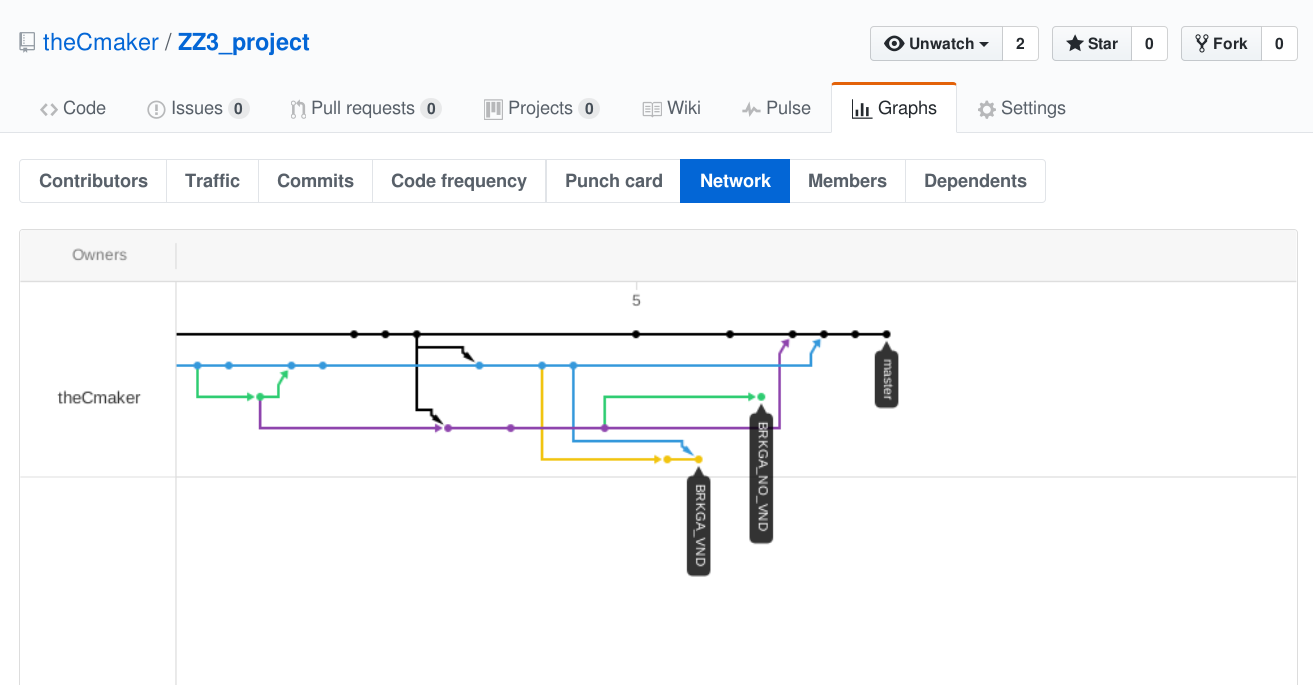
\includegraphics[width=\linewidth]{git}
			\caption{Gestion de branches avec Git}
			\label{fig:git}
		\end{figure}

		\begin{figure}[h!]
			\centering
			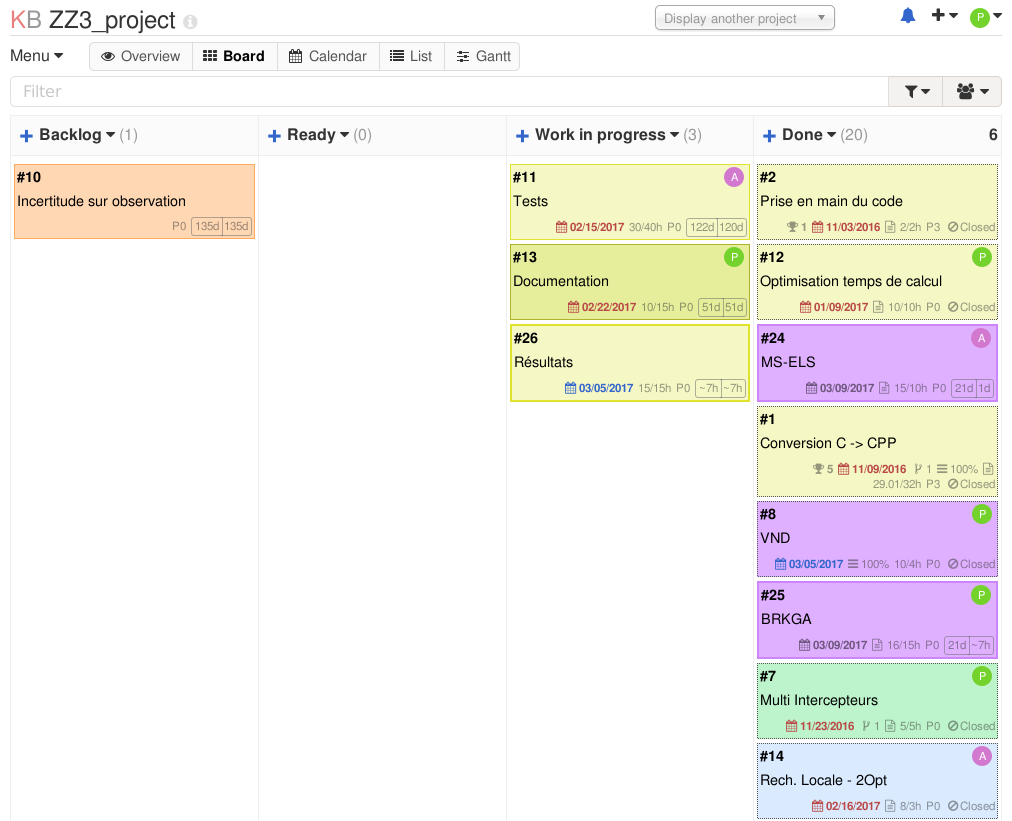
\includegraphics[width=\linewidth]{dashboard}
			\caption{Dashboard de gestion de projet de type Kanban}
			\label{fig:dashboard}
		\end{figure}


  \chapter{Résultats}
    \section{Avant améliorations}
    	Résultats depuis le passage au C++, le gain en temps avec le cache, les corrections et améliorations des heuristiques de construction.
    	Comparaison avec les résultats ZZ1.
    \section{Après améliorations}
    	Résultats de la VND
    	Résultats du MS-ELS
    	Résultats du BRKGA
    \section{Perspectives}
    
    	\begin{itemize}
    		\item amélioration du MS-ELS (critère de sélection des meilleures solutions -> il favorise pour l'instant le temps et donne des résultats moins bons + problème du mono critère)
    		\item ajout de l'incertitude (loi de Poisson ou loin exponentielle négative ?)
    		\item multi-thread des métaheuristiques pour augmenter les performances de calcul
    	\end{itemize}
    		


  % Conclusion
  \chapter*{Conclusion}
\addcontentsline{toc}{chapter}{Conclusion}

La conception et l'optimisation d'algorithmes pour résoudre des problèmes NP-Difficiles tels que le \acrlong{vrp} sont des pratiques courantes d'aide à la décision. Pour ce projet, nous étions chargés de concevoir un solveur pour un \acrlong{stdvrp} à l'aide de méthodes itératives et en reprenant un projet existant. Il consistait à atteindre le maximum d'objets mobiles dans un espace plat à l'aide d'un ou plusieurs intercepteurs. Ce problème s'inscrit dans un objectif bi-critère où l'on cherche autant à intercepter le plus grand nombre de mobiles qu'à réduire au maximum le coût en temps.

Pour cela, les heuristiques de constructions déjà présentes ont été traduites en C++, intégrées dans un modèle objet et optimisée pour obtenir des résultats plus performants. Puis une recherche locale, la VND, constituée de huit mouvements au sein d'une ou plusieurs tournées a été intégrée dans le but d'améliorer les solutions générées. Deux métaheuristiques ont ensuite été ajoutées pour perfectionner les résultats : la \acrlong{msels} et un algorithme génétique, le \acrlong{brkga}.

Les résultats obtenus sont encourageants, notamment ceux du BRKGA, car ils montrent qu'il est possible de calculer dans un temps raisonnable de bonnes solutions, permettant à la fois de rater peu de mobiles et d'optimiser le temps d'interception de la pire tournée.

Ainsi, il serait intéressant de poursuivre ce projet en y apportant quelques corrections pour améliorer encore plus les résultats et le temps de calcul. Avec une meilleure agrégation des deux critères du problème, la MS-ELS pourrait donner de meilleures solutions. L'ajout de nouvelles métaheuristiques ainsi que le passage à un programme multi-threadé permettraient aussi d'obtenir un pannel plus large pour la recherche de solutions optimales dans un temps polynomial.


  % Glossaire
  \cleardoublepage
  \pagenumbering{roman}                   % Retour chiffres romains
  \setcounter{page}{\value{oldRomanNum}}  % Récupération du numéro de page
  \printglossary[title=Glossaire]
  
  %Webographie
  \cleardoublepage
  \renewcommand{\bibname}{Webographie}
\begin{thebibliography}{9}
  \addcontentsline{toc}{chapter}{Webographie}
  \bibitem[Nom]{labelCite}
    \emph{Titre}\\
    \url{http://www.example.net}\\
    Consulté le \TODO{Date de consultation.}
\end{thebibliography}

  %Annexes
  \cleardoublepage
  \appendix
  \pagenumbering{Roman}
  \chapter{Réalisation d'une politique de cache de données}
\label{app:cache}
	L'utilisation d'un \gls{cache} permet de stocker des informations et de les conserver jusqu'au moment où l'on souhaite y accéder.

	Dans notre heuristique d'insertion au plus tôt, nous sommes contraints de déterminer après chaque interception quel est le mobile suivant qui pourra être intercepté au plus tôt. Une interception concerne uniquement un mobile et un intercepteur. Ainsi dans un problème à $n$ mobiles et $m$ intercepteurs, à la première interception, ce sont $n-1$ mobiles et $m-1$ intercepteurs ne seront pas concernés, soit $n \times m -n -m +1$ dates d'interception potentielles qui resteront les mêmes au calcul de la seconde interception.

	Le calcul des dates d'interception fait appel à plusieurs fonctions trigonométriques et demande donc un temps plus important que pour effectuer des calculs élémentaires. Il est par conséquent impératif de faire le maximum pour réduire le nombre d'appels à ce calcul. Sachant que l'on travaille avec $n$ mobiles et $m$ intercepteurs, il suffit de conserver entre chaque interception une matrice des dates d'interception. Il s'agit précisément du principe de cache. Le contrôle de l'obsolescence des données de ce cache est simple à définir: les dates d'interception pour un mobile ne sont plus d'aucune utilité lorsque ce dernier est intercepté, et les dates d'interception de tous les mobiles non-interceptés pour un intercepteur doivent être recalculées lorsque ce dernier change de position, c'est-à-dire lorsqu'il réalise une interception. Dans ce dernier cas, il convient de mettre à jour les données en cache pour les mobiles qui ne sont pas encore interceptés.

	Le schéma de la figure \ref{fig:cache} détaille les opérations sur le cache selon les différentes étapes du diagramme de séquences de la figure \ref{diag:cache}.

	\TODO{fig:cache}
	\TODO{diag:cache}

	Dans notre implémentation, nous avons donc proposé deux politiques: la première dépourvue de cache et la seconde fournissant les fonctionnalités décrites plus haut. Ces deux politiques sont décrites selon le diagramme UML de la figure \ref{uml:cache_policies}.

\chapter{Seconde annexe}

\end{document}